%%%%%%%%%%%%%%%%%%%%%%%%%%%%%%%%%%%%%%%%%%%%%%%%%%%%%%%%%%%%%%%%%%%%%%
% Lớp 11 | Quan hệ vuông góc trong không gian | Hình lăng trụ đứng. Hình chóp đều. Thể tích
% Dạng 1H8?7-9: Toán thực tế hình lăng trụ đứng, chóp đều, thể tích
% Số câu: 11  (sinh tự động bởi tach_cau.py; từ nay thầy sửa trực tiếp file này)
%%%%%%%%%%%%%%%%%%%%%%%%%%%%%%%%%%%%%%%%%%%%%%%%%%%%%%%%%%%%%%%%%%%%%%

%%%%%%%%%%%%%%%% TRẢ LỜI NGẮN %%%%%%%%%%%%%%%%

% nguồn: Ok_TraLoiNgan_Lop11_Lan2
\begin{ex}%[1H8H7-9]%[ma:621eab56]
	\immini{Một khối rubik $3\times3$ (được chia làm $27$ khối lập phương nhỏ) có dạng một hình lập phương với kích thước cạnh bằng  $6$ cm. Tìm thể tích của khối rubik đó, biết khoảng hở giữa các khối lập phương nhỏ
	không đáng  kể.}
	 {\pgfmathsetmacro\radius{0.1}
	 \newcommand{\frontcolor}{red}
	 \newcommand{\sidecolor}{blue}
	\tdplotsetmaincoords{55}{135} 
	\begin{tikzpicture}
			 \clip (-3,-2.5) rectangle (3,2.5);
			\begin{scope}[tdplot_main_coords]
				\filldraw [canvas is yz  plane at x=1.5] (-1.5,-1.5) rectangle (1.5,1.5);
				\filldraw [canvas is xz plane  at y=1.5] (-1.5,-1.5) rectangle (1.5,1.5);
				\filldraw [canvas is yx plane at z=1.5] (-1.5,-1.5) rectangle (1.5,1.5); 
				\foreach \X in  {-1.5,-0.5,0.5}{
					\foreach \Y in  {-1.5,-0.5,0.5}{
					\draw [thick,canvas is yz plane at x=1.5,shift={(\X,\Y)},fill=\sidecolor] (0.5,0) -- ({1-\radius},0) arc (-90:0:\radius) -- (1,{1-\radius})  arc (0:90:\radius) -- (\radius,1) arc (90:180:\radius) -- (0,\radius) arc (180:270:\radius) -- cycle;
					\draw [thick,canvas is xz plane at y=1.5,shift={(\X,\Y)},fill=\frontcolor] (0.5,0) --  ({1-\radius},0) arc (-90:0:\radius) -- (1,{1-\radius}) arc (0:90:\radius) -- (\radius,1) arc (90:180:\radius) -- (0,\radius) arc (180:270:\radius) -- cycle;
					\draw [thick,canvas is yx plane at z=1.5,shift={(\X,\Y)},fill=yellow] (0.5,0) -- ({1-\radius},0) arc (-90:0:\radius) -- (1,{1-\radius}) arc  (0:90:\radius) -- (\radius,1) arc (90:180:\radius) -- (0,\radius) arc (180:270:\radius) -- cycle;
				 }
				 }
			\end{scope}
		\end{tikzpicture}
	} 
	\shortans{116} 
	 \loigiai{
		Thể tích khối rubik là  $V=6^3=116$ (cm$^3$).
	} 
\end{ex}

% nguồn: Ok_TraLoiNgan_Lop11_Lan2
\begin{ex}%[1H8V7-9]%[ma:a8bcc5db]
	Hình bên là hình chụp đền Kukulcan, là một kim tự tháp Trung Mỹ nằm ở khu di tích Chichen Itza, Mexico, được người Maya xây vào khoảng từ thế kỉ $IX$ đến thế kỉ $XII$. Phần thân của đền, không bao gồm đền nằm phía trên, có dạng một khối chóp cụt tứ giác đều (không tính cầu thang và coi các mặt bên là phẳng) với độ dài đáy dưới là $55{,}3$ (m), chiều cao là $24$ (m), góc phẳng nhị diện tạo bởi mặt bên và mặt đáy là $\alpha$. Tính thể tích phần thân ngôi đền có dạng khối  chóp cụt tứ giác đều đó theo đơn vị decametre khối (\textit{làm tròn kết quả đến hàng phần mười}), biết rằng $\tan\alpha=\dfrac{320}{211}$.
	\shortans{39,4} 
	 \loigiai{
	\immini{Giả sử  khối chóp cụt tứ giác đều cần tính thể tích là $ABCD.A'B'C'D'$ có $O$, $O'$ lần lượt là tâm của hai đáy. Gọi $M$, $M'$ lần lượt là trung điểm của $BC$, $B'C'$ như hình vẽ; $H$ là hình chiếu vuông góc của $M'$ lên $OM$.\\
		Khi đó góc phẳng  nhị diện của mặt bên $ADD'A'$ và mặt đáy $ABCD$ là góc $\widehat{M'MH}=\alpha$.\\
		Ta có $\tan\widehat{M'MH}=\dfrac{M'H}{MH}=\dfrac{24}{MH}=\dfrac{320}{211}\\\Rightarrow  MH=\dfrac{24\cdot211}{320}=\dfrac{633}{40}$.\\
		$\Rightarrow  A'B'=2\cdot O'M'=2(OM-HM)=55{,}3-\dfrac{633}{20}=\dfrac{473}{20}=23{,}65$.\\
		Do đó thể tích  phần thân đền bằng\\
		}{ 
		\begin{tikzpicture}[declare function={goc=-150; a=3.5; b=a/2; h=6;}]
				 \path (0,0) coordinate (A)
					 (a,0) coordinate (B)
					(goc:b) coordinate (D) 
					+(a,0) coordinate (C) 
					($(A)!.5!(C)$) coordinate (O) 
					+(0,h) coordinate (S) 
					 ($(A)!.4!(S)$) coordinate (A')
					($(B)!.4!(S)$) coordinate  (B')
					 ($(C)!.4!(S)$) coordinate (C')
					 ($(D)!.4!(S)$) coordinate (D')
					($(A')!.5!(C')$)  coordinate (O')
					($(A)!.5!(D)$) coordinate (M) 
					($(A')!.5!(D')$)  coordinate (M')
					 ($(O)!(M')!(M)$) coordinate (H);
				\draw pic[angle radius=2mm,draw] {right angle = S--O--D}; 
				\draw pic[angle radius=2mm,draw] {right angle = D'--O'--O}; 
				\draw[dashed]  (A')--(A)
					(D)--(A)--(B) 
					 (O')--(O)
					(A)--(C) 
					 (D)--(B)
					(A)--(D) 
					 (M)--(M')
					 (O)--(M)
					 (M')--(H);
				\draw (D)--(C)--(B)--(B')--(C')--(D')--(A')--(B') 
					 (C)--(C')
					(D)--(D') 
					 (A')--(C')
					 (D')--(B')
					(O')--(M'); 
				\foreach \x/\goc  in {A/30,B/0,C/-60,D/-180,O/-90,A'/90,B'/90,C'/90,D'/90,O'/90,M/180,M'/90,H/-140}
				\draw[fill=white] (\x) node[shift={(\goc:7pt)},font=\scriptsize]{$\x$}  circle (1pt);
			\end{tikzpicture}
		} 
		$V=\dfrac{OO'}{3}\cdot\left(AB^2+A'B'^2+AB\cdot  A'B'\right)=\dfrac{24}{3}\left(55{,}3^2+23{,}65^2+55{,}3\cdot23{,}65\right)\approx 39{,}4$ (dam$^3$).
	 }
\end{ex}

% nguồn: Ok_TraLoiNgan_Lop11_Lan2
\begin{ex}%[1H8V7-9]%[ma:4fda1fa2]
	\immini{Một loại đèn đá muối có dạng khối chóp tứ giác đều (hình bên). Tính theo thể tích của đèn đá muối đó, giả sử các cạnh đáy và các cạnh bên đều bằng $5$ (\textit{làm tròn kết quả đến hàng phần mười}).}{\begin{tikzpicture}[declare function={goc=-150; a=3.5; b=a/2; h=4;}]
		\path (0,0)  coordinate (A)
			(a,0)  coordinate (B)
			(goc:b)  coordinate (D)
			 +(a,0) coordinate (C)
			($(A)!.5!(C)$) coordinate  (O)
			+(0,h)  coordinate (S);
		\draw pic[angle  radius=3mm,draw] {right angle = S--O--D};
		\draw[dashed] (S)--(A) 
			(D)--(A)--(B) 
			(S)--(O) 
			(A)--(C) 
			(D)--(B); 
		\draw (S)--(D)--(C)--(S)--(B)--(C)--cycle; 
		\foreach \x/\goc  in {S/90,A/150,B/0,C/-60,D/-180,O/-90}
		\draw[fill=white] (\x) node[shift={(\goc:7pt)},font=\scriptsize]{$\x$} circle  (1pt);
	\end{tikzpicture}
	} 
	 \shortans{29,5}
	 \loigiai{
		 Mô hình hoá đèn đá muối bằng hình chóp tứ giác đều $S.ABCD$.\\
		Gọi $O$ là tâm  của đáy.
		\begin{itemize}
			\item $\triangle SAC$ cân tại $S\Rightarrow SO\perp  AC$.
			 \item $\triangle SBD$ cân tại $S\Rightarrow SO\perp BD\Rightarrow SO\perp(ABCD)$.
			\item $ABCD$ là hình vuông $\Rightarrow AC=\sqrt{AB^2+BC^2}=5\sqrt{2}\Rightarrow AO=\dfrac{1}{2}AC=\dfrac{5\sqrt{2}}{2}$. 
			\item $\triangle SAO$ vuông tại  $O\Rightarrow SO=\sqrt{SA^2-AO^2}=\dfrac{5\sqrt{2}}{2}$.
			 \item $S_{ABCD}=AB^2=5^2$.
			 \item $V_{S.ABCD}=\dfrac{1}{3}\cdot S_{ABCD}\cdot SO=\dfrac{5^3\sqrt{2}}{6}\approx 29{,}5$.
		\end{itemize}
	 }
\end{ex}

% nguồn: Ok_TraLoiNgan_Lop11_Lan2
\begin{ex}%[1H8V7-9]%[ma:64da361b]
	Một chiếc tháp có phần dưới có dạng hình hộp chữ nhật, đáy là hình vuông có cạnh dài $5$ m. chiều cao của hình hộp chữ nhật là $12$ m. Phần trên của tháp có  dạng hình chóp đều, các mặt bên là các tam giác cân chung đỉnh. Mỗi cạnh bên của hình chóp dài $8$ m. Tính thể tích của tháp đồng hồ này (\textit{làm tròn kết quả đến hàng đơn vị}).
	 \shortans{360}
	\loigiai{ 
	\immini{Xét hình vuông $A'B'C'D'$ có\\  $B'D'=\sqrt{B'C'^2+C'D'^2}=\sqrt{5^2+5^2}=5\sqrt{2}\\\Rightarrow O'D'=\dfrac{5\sqrt{2}}{2}$.\\
		Chiều  cao phần trên của tháp\\ $SO'=\sqrt{SD'^2-O'D'^2}=\sqrt{8^2-\left( \dfrac{5\sqrt{2}}{2}\right)^2}=\dfrac{\sqrt{206}}{2}$.\\
		Thể tích phần  dưới của tháp\\ $V_1=S_{ABCD}\cdot OO'=5^2\cdot12=300$ (m$^3$).\\
		Thể tích phần trên của tháp\\ $V_2=\dfrac{1}{3}S_{A'B'C'D'}\cdot  SO'=\dfrac{1}{3}\cdot5^2\cdot\dfrac{\sqrt{206}}{2}=\dfrac{25\sqrt{206}}{6}$ (m$^3$).\\
		Thể tích của tháp $V_1+V_2=300+\dfrac{25\sqrt{206}}{6}\approx 360$  (m$^3$).}{
		\begin{tikzpicture}[declare function={r=3.5; l=5; h=3;},font=\scriptsize]
				 \path (0:0) coordinate (B)
					(0:r)  coordinate (C)
					 ++(37:{0.65*r}) coordinate (D)
					++(180:r) coordinate  (A)
				 \foreach \x in {A,B,C,D}{(\x)++(90:l) coordinate (\x_1)}
					(intersection of  A--C and B--D) coordinate (O)
					 (intersection of A_1--C_1 and B_1--D_1) coordinate (O')+(0,h) coordinate (S)
					($(B)!0.5!(C)$)  coordinate (E) node[below]{$5$ m}
					($(B)!0.5!(B_1)$)  coordinate (F) node[left]{$12$ m}
					 ($(S)!0.5!(D_1)$) coordinate (G) node[right]{$8$ m};
				\draw[dashed] (A_1)--(D_1) 
					 (S)--(A_1)
					 (A)--(B)
					 (D)--(A)
					 (A)--(C)
					(B)--(D) 
					(O)--(S) 
					 (A_1)--(C_1)
					 (B_1)--(D_1)
					(A_1)--(B_1) 
					 (A)--(A_1);
				 \draw (B)--(C)
					 (D)--(C)
					 (B)--(B_1)
					 (C)--(C_1)
					 (B_1)--(C_1)--(D_1)
					(D_1)--(D) 
					(S)--(B_1) 
					(S)--(C_1) 
					 (S)--(D_1);
				\foreach \x/\goc/\t  in {A/180/A,B/180/B,C/0/C,D/0/D,A_1/135/A',B_1/180/B',
					C_1/0/C',D_1/0/D',O/-90/O,O'/40/O',S/90/S}{ 
					\draw[fill=white] (\x)  circle (1pt) node[shift={(\goc:9pt)}]{$\t$};
				 }
			\end{tikzpicture}
		 }
	 }
\end{ex}

% nguồn: Ok_TraLoiNgan_Lop11_Lan2
\begin{ex}%[1H8V7-9]%[ma:a6b527a9]
	Người  ta định đào một cái hầm có dạng hình chóp cụt tứ giác đều có hai cạnh đáy là $14$ m và $10$ m.
	Mặt bên tạo với đáy nhỏ thành một góc nhị diện có số đo bằng  $135^{\circ}$. Tính số mét khối đất cần phải di
	chuyển ra khỏi hầm  (hình bên dưới) (\textit{làm tròn kết quả đến hàng phần đơn vị}).
	 \shortans{291}
	\loigiai{Gọi $O$, $O'$, $M$, $M'$ lần lượt là tâm hai đáy và trung  điểm hai cạnh đáy lớn và đáy nhỏ tương ứng.
	 \immini{
		Vẽ  đường cao $M'H$ của hình thang vuông $OMM'O'$.\\
		 Ta có $\widehat{MMO'}=135^{\circ}$, $\widehat{M'MO}=45^{\circ}$,\\
		$OO'=HM'=(OM-O'M')\cdot\tan\widehat{M'MO}=(7-5)\cdot\tan  45^{\circ}=2$.\\
		$V=\dfrac{1}{3}h(S+\sqrt{SS'}+S')=\dfrac{1}{3}\cdot2\cdot(14^{2}+14\cdot10+10^{2})\approx  291$ (m$^3$).\\
		Vậy cần phải di chuyển ra khỏi hầm  khoảng $291$ (m$^3$).}{
		\begin{tikzpicture}[declare function={goc=-150; a=3.75; b=a/2; h=6;}]
				\path  (0,0) coordinate (A)
					(a,0) coordinate (B) 
					(goc:b) coordinate  (D)
					+(a,0)  coordinate (C)
					($(A)!.5!(C)$) coordinate (O) 
					+(0,h) coordinate (S) 
					($(A)!.4!(S)$)  coordinate (A')
					($(B)!.4!(S)$) coordinate  (B')
					($(C)!.4!(S)$) coordinate  (C')
					($(D)!.4!(S)$) coordinate (D') 
					($(A')!.5!(C')$) coordinate  (O')
					 ($(A)!.5!(D)$) coordinate (M)
					($(A')!.5!(D')$) coordinate (M') 
					($(O)!(M')!(M)$)  coordinate (H);
				\draw pic[angle radius=2mm,draw] {right angle =  S--O--D};
				\draw pic[angle radius=2mm,draw]  {right angle = D'--O'--O};
				 \draw[dashed] (A')--(A)
					 (D)--(A)--(B)
					 (O')--(O)
					 (A)--(C)
					 (D)--(B)
					 (A)--(D)
					 (M)--(M')
					(O)--(M) 
					(M')--(H); 
				\draw  (D)--(C)--(B)--(B')--(C')--(D')--(A')--(B')
					 (C)--(C')
					(D)--(D') 
					 (A')--(C')
					 (D')--(B')
					 (O')--(M');
				 \foreach \x/\goc in {A/30,B/0,C/-60,D/-180,O/-90,A'/90,B'/90,C'/90,D'/90,O'/90,M/180,M'/90,H/-140}
				 \draw[fill=white] (\x) node[shift={(\goc:7pt)},font=\scriptsize]{$\x$} circle (1pt);
			\end{tikzpicture}
		} 
	} 
\end{ex}

% nguồn: Ok_TraLoiNgan_Lop11_Lan2
\begin{ex}%[1H8V7-9]%[ma:e73a712f]
	\immini{Người ta cần đổ bê tông để  làm những viên gạch có dạng khối lăng trụ lục giác đều (hình bên dưới)
	với chiều cao  là $4$ cm và cạnh lục giác dài $21{,}5$ cm. Tính thể tích bê tông theo đơn vị centimét khối
	để làm một viên gạch như thế  (\textit{đơn vị $\mathrm{cm}$, làm tròn kết quả đến hàng đơn vị}).}{
	\begin{tikzpicture}[join = round,cap = round,smooth,font = \small,scale =.8]
			\def\a{2.5} 
			 \path
				(0:0) coordinate (E) 
				--(0:\a)  coordinate (D)
				--([turn]60:\a)  coordinate (C)
				--([turn]60:\a) coordinate (B) 
				--([turn]60:\a) coordinate  (A)
				--([turn]60:\a) coordinate  (F)
				 (barycentric cs:A=1,B=1,C=1,D=1,E=1,F=1) coordinate (O);
			\path (A) [shift = (30:1)] coordinate (A1) 
				(B) [shift = (30:1)] coordinate  (B1)
				 (C) [shift = (30:1)] coordinate (C1)
				(D)  [shift = (30:1)] coordinate (D1)
				 (E) [shift = (30:1)] coordinate (E1)
				(F)  [shift = (30:1)] coordinate (F1);
			 \path ($(C)!0.5!(C1)$) coordinate (G)
				($(C1)!1.25!-150:(G)$) coordinate  (H)
				($(H)!1.5!120:(C1)$) coordinate (I); 
			 \draw
				(A)--(B)--(C)--(D)--(E)--(F)--cycle 
				 (A)--(A1)--(B1)--(C1)--(D1)--(D)
				(B)--(B1) 
				 (C)--(C1)
				(G)--(H)--(I); 
			\draw (A1)--(B1) node[midway,above]{$21{,5}$  cm};
			\draw (H)--(I) node[midway,above]{$4$ cm}; 
			\draw[dashed](A1)--(F1)--(E1)--(D1) 
				 (F)--(F1)
				(E)--(E1); 
		\end{tikzpicture}
	 }
	\shortans{4804} 
	\loigiai{ 
		Chia  hình lục giác đều trên hai mặt đáy thành $6$ hình tam giác đều cạnh $21{,}5$ cm.\\
		Khi  đó diện tích đáy của viên gạch bằng $6\cdot\dfrac{(21{,}5)^2\cdot\sqrt{3}}{4}=\dfrac{5\,547\sqrt{3}}{8}$ (cm$^2$).\\ Thể tích bê tông cần dùng bằng thể tích viên gạch, tức là $\dfrac{5\,547\sqrt{3}}{2}\approx 4\,804$ (cm$^3$).
	} 
\end{ex}

% nguồn: Ok_TraLoiNgan_Lop11_Lan2
\begin{ex}%[1H8V7-9]%[ma:6311fd36]
	\immini{Hình bên dưới là hình chụp đền Kukulcan, là một kim tự tháp Trung Mỹ nằm ở khu di tích Chichen Itza, Mexico, được người Maya xây vào khoảng từ thế kỉ $IX$ đến thế kỉ $XII$. Phần thân của đền, không bao gồm ngôi đền nằm phía trên, có dạng một khối chóp cụt tứ giác đều (không tính cầu thang và coi các mặt bên là phẳng) với độ dài đáy dưới là $55{,}3$ m, chiều cao là $24$ m, góc giữa cạnh  bên và mặt phẳng đây là khoảng $47^{\circ}$. Tính thể tích phần thân ngôi đền có dạng khối chóp cụt tứ giác đều đó theo đơn vị decametre khối
	(\textit{làm tròn kết quả đến hàng phần mười}).}{\begin{tikzpicture}[declare function={goc=-150; a=4; b=a/2; h=6;}]
		\path  (0,0) coordinate (A)
			 (a,0) coordinate (B)
			(goc:b) coordinate  (D)
			+(a,0) coordinate (C) 
			($(A)!.5!(C)$) coordinate (O) 
			 +(0,h) coordinate (S)
			($(A)!.4!(S)$) coordinate  (A')
			($(B)!.4!(S)$)  coordinate (B')
			($(C)!.4!(S)$) coordinate  (C')
			 ($(D)!.4!(S)$) coordinate (D')
			 ($(A')!.5!(C')$) coordinate (O')
			($(O)+(C')-(O')$) coordinate  (H);
		\draw  (D)--(C)--(B)--(B')--(C')--(D')--(A')--(B')
			 (C)--(C')
			 (D)--(D');
	\end{tikzpicture}
	} 
	 \shortans{39,4}
	 \loigiai{
		\begin{center}
			\begin{tikzpicture}[declare function={goc=-150; a=5; b=a/2; h=6;}]
					\path (0,0) coordinate  (A)
						(a,0) coordinate (B) 
						(goc:b)  coordinate (D)
						+(a,0) coordinate (C) 
						 ($(A)!.5!(C)$) coordinate (O)
						+(0,h)  coordinate (S)
						($(A)!.4!(S)$) coordinate (A') 
						($(B)!.4!(S)$) coordinate  (B')
						($(C)!.4!(S)$)  coordinate (C')
						($(D)!.4!(S)$)  coordinate (D')
						($(A')!.5!(C')$) coordinate  (O')
						($(O)+(C')-(O')$) coordinate  (H);
					\draw pic[angle  radius=2mm,draw] {right angle = S--O--D};
					\draw pic[angle radius=2mm,draw] {right angle =  D'--O'--O};
					\draw[dashed] (A')--(A) 
						 (D)--(A)--(B)
						 (O')--(O)
						 (A)--(C)
						 (D)--(B)
						(A)--(D) 
						 (C')--(H);
					\draw  (D)--(C)--(B)--(B')--(C')--(D')--(A')--(B')
						 (C)--(C')
						(D)--(D') 
						(A')--(C') 
						 (D')--(B');
					 \foreach \x/\goc in {A/150,B/0,C/-60,D/-180,O/-90,A'/90,B'/90,C'/90,D'/90,O'/90,H/30}
					\draw[fill=white] (\x)  node[shift={(\goc:7pt)},font=\scriptsize]{$\x$} circle (1pt);
				\end{tikzpicture}
		\end{center}
		Mô hình hoá phần thân của đền bằng hình chóp cụt tứ giác đều $ABCD.A'B'C'D'$ với $O$, $O'$ là tâm  của hai đáy.\\ Vậy $AB=55{,}3$; $OO'=24$; $(CC',(ABCD))=47^{\circ}$.\\
		$ABCD$ là hình vuông 
		$\Rightarrow  AC=\sqrt{AB^2+BC^2}=55{,}3\sqrt{2}\Rightarrow CO=\dfrac{1}{2}AC=27{,}65\sqrt{2}$.\\
		Kẻ $C'H\perp OC\,\,(H\in OC)\Rightarrow  C'H\parallel OO'\Rightarrow C'H\perp(ABCD)$.\\
		$\Rightarrow(CC',(ABCD))=(CC',CH)=\widehat{HCC}=47^{\circ}$.\\ 
		$OHC'O'$  là hình chữ nhật $\Rightarrow OO'=C'H=24$, $OH=O'C'$.\\
		 $\triangle C'CH$ vuông tại $H\Rightarrow CH=\dfrac{C'H}{\tan\widehat{HCC}}=\dfrac{24}{\tan 47^{\circ}}$.\\
		 $O'C'=OH=CO-CH=27{,}65\sqrt{2}-\dfrac{24}{\tan 47^{\circ}}\Rightarrow A'C'=2O'C'=2\cdot\left(27{,}65\sqrt{2}-\dfrac{24}{\tan 47^{\circ}}\right)$.\\
		 $A'B'C'D'$ là hình vuông $\Rightarrow A'B'=\dfrac{A'C'}{\sqrt{2}}=55{,}3-\dfrac{24\sqrt{2}}{\tan 47^{\circ}}$.\\
		Diện tích đáy lớn  là $S=AB^2=55{,}3^2$ (m$^2$).\\
		Diện tích đáy bé là $S'=A'B'^2=\left(55{,}3-\dfrac{24\sqrt{2}}{\tan 47^{\circ}}\right)^2$  (m$^2$).\\
		Thể tích hình chóp cụt  là\\
		 $V=\dfrac{1}{3}h\cdot\left(S+\sqrt{SS'}+S'\right)\approx 39\,401{,}6
		$  (m$^3$).\\
		Vậy  thể tích phần thân ngôi đền có dạng khối chóp cụt từ giác đều đó là
		$39{,}4$ (dam$^3$). 
	 }
\end{ex}

% nguồn: Ok_TraLoiNgan_Lop11_Lan2
\begin{ex}%[1H8V7-9]%[ma:a9e2e1ff]
	Người ta xây dựng một chân tháp bằng  bê tông có dạng khối chóp cụt tứ giác đều (hình bên dưới). Cạnh đáy dưới dài $5$ m, cạnh đáy trên dài $2$ m, cạnh bên dài $3$ m. Biết rằng chân tháp được làm bằng bê tông tươi với giá tiền là $1\,470\,000$ đồng/m$^3$. Tính số tiền để mua bê tông tươi làm chân tháp theo đơn vị triệu đồng (\textit{làm tròn kết quả đến hàng triệu}).
	 \shortans{41}
	\loigiai{ 
	\immini{Theo đề ta có $AB=5$,  $A'B'=2$, $CC'=3$.\\
		Ta có $ABCD$ là  hình vuông $\Rightarrow CO=\dfrac{1}{2}AC=\dfrac{5\sqrt{2}}{2}$.\\
		Lại có  $A'B'C'D'$ là hình vuông nên\\
		 $A'C'=\sqrt{A'B'^{2}+B'C'^{2}}=2\sqrt{2}\Rightarrow C'O'=\dfrac{1}{2}A'C'=\sqrt{2}$.\\
		Kẻ $C'H\perp OC\Rightarrow OHC'O'$ là hình chữ nhật\\ 
		 $\Rightarrow OH=O'C'=\sqrt{2}$, $OO'=C'H=CH=OC-OH=\dfrac{3\sqrt{2}}{2}$.\\
		Mặt khác tam  giác $CC'H$ vuông tại $H$ nên \\
		$C'H=\dfrac{3\sqrt{2}}{2}\Rightarrow OO'=C'H=\dfrac{3\sqrt{2}}{2}$.\\ 
		Diện tích đáy lớn là $S=AB^2=5^2=25$ (m$^2$).\\ 
		Diện tích đáy bé  là $S'=A'B'^2=2^2=4$ (m$^2$).
		}{\begin{tikzpicture}[declare function={goc=-150; a=4; b=a/2; h=6;}]
		\path (0,0) coordinate  (A)
			(a,0) coordinate (B) 
			(goc:b)  coordinate (D)
			+(a,0)  coordinate (C)
			($(A)!.5!(C)$) coordinate (O) 
			+(0,h) coordinate (S) 
			 ($(A)!.4!(S)$) coordinate (A')
			 ($(B)!.4!(S)$) coordinate (B')
			 ($(C)!.4!(S)$) coordinate (C')
			($(D)!.4!(S)$) coordinate  (D')
			($(A')!.5!(C')$) coordinate  (O');
		\draw pic[angle radius=2mm,draw] {right angle =  S--O--D};
		\draw pic[angle radius=2mm,draw] {right angle = D'--O'--O}; 
		\draw[dashed]  (A')--(A)--(D)
			 (D)--(A)--(B)
			 (O')--(O)
			(A)--(C) 
			(D)--(B); 
		\draw  (D)--(C)--(B)--(B')--(C')--(D')--(A')--(B')
			(C)--(C') 
			(D)--(D') 
			 (A')--(C')
			 (D')--(B');
		\foreach \x/\goc  in {A/40,B/0,C/-60,D/-180,O/-90,A'/180,B'/0,C'/0,D'/180,O'/90}
		\draw[fill=white] (\x) node[shift={(\goc:7pt)},font=\scriptsize]{$\x$} circle (1pt); 
	\end{tikzpicture}
		} 
		 \noindent Thể tích hình chóp cụt là
		$V=\dfrac{1}{3}h\left(S+\sqrt{SS'}+S'\right)=\dfrac{1}{3}\cdot\dfrac{3\sqrt{2}}{2}\cdot\left(25+\sqrt{25\cdot4}+4\right)=\dfrac{39\sqrt{2}}{2}$  (m$^3$).\\
		Số tiền để mua bê  tông tươi làm chân tháp là $\dfrac{39\sqrt{2}}{2}\cdot1\,470\,000\approx 40\,538\,432\approx 41$ (triệu đồng).
	 }
\end{ex}

% nguồn: Ok_TraLoiNgan_Lop11_Lan2
\begin{ex}%[1H8V7-9]%[ma:4d2e2de6]
	\immini{Một cái hộp hình lập phương, bên trong nó đựng một mô hình đồ chơi có dạng hình chóp tứ giác đều mà đỉnh của hình chóp đó trùng với tâm của một mặt chiếc hộp, giả sử hình vuông đáy của hình chóp trùng với một mặt của chiếc hộp (mặt này cùng với mặt chứa đỉnh hình chóp là hai mặt đối nhau). Biết cạnh của chiếc hộp bằng $30$ cm, hãy tính thể tích phần không gian bên trong chiếc hộp không bị chiếm bởi mô hình đồ chơi dạng hình chóp (mô hình đồ chơi được làm bởi chất liệu nhựa đặc bên trong, đơn vị dm$^3$).}{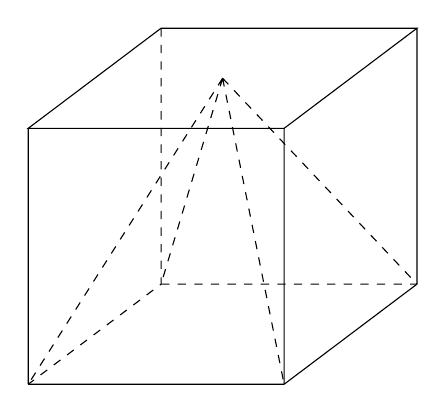
\begin{tikzpicture}[declare function={r=3.25;},font=\scriptsize]
		\path  (0:0) coordinate (A)
			(0:r) coordinate (B) 
			++(37:{0.65*r})  coordinate (C)
			++(180:r) coordinate (D) 
		\foreach \x in {A,B,C,D}{(\x)++(90:r) coordinate  (\x_1)}
			(intersection of A_1--C_1 and B_1--D_1) coordinate (G); 
		\draw[dashed] (D_1)--(D)--(A) 
			 (D)--(C)
			(G)--(A) 
			(G)--(B) 
			(G)--(C) 
			(G)--(D); 
		 \draw (A)--(B)--(C)
			 (A)--(A_1)
			(B)--(B_1) 
			(C)--(C_1) 
			 (A_1)--(B_1)--(C_1)--(D_1)--cycle;
	\end{tikzpicture}
	} 
	 \shortans{18}
	\loigiai{ 
		Thể tích cái hộp (khối lập  phương) là $V_1=30^3=27\,000$ (cm$^3$).\\
		Xét đồ chơi có dạng hình chóp tứ giác đều, chiều cao của hình chóp  bằng với một cạnh của hình
		lập phương, hay $h=30$ cm, đáy của hình  chóp có diện tích $S=30^2=900$ (cm$^2$).\\
		Thể tích khối đồ chơi (khối  chóp tứ giác đều) là
		 $V_2=\dfrac{1}{3}Sh=\dfrac{1}{3}\cdot900\cdot30=9\,000$ (cm$^3$).\\
		Thể tích phần không gian  bên trong chiếc hộp không bị chiếm bởi mô hình đồ chơi dạng hình chóp
		$V=V_1-V_2=27\,000-9\,000=18\,000$ (cm$^3$) =  $18$ (dm$^3$).
	} 
\end{ex}

% nguồn: Ok_TraLoiNgan_Lop11_Lan2
\begin{ex}%[1H8V7-9]%[ma:2d2a6be9]
	Người ta dự định đào một hầm rượu có dạng hình chóp cụt đều có hai cạnh đáy là  $7$ m và $5$ m. Mặt bên
	tạo với đáy nhỏ thành một góc nhị  diện có số đo bằng $120^{\circ}$. Tính số mét khối đất cần phải di chuyển ra khỏi hầm (\textit{đơn vị $\mathrm{m}$, làm tròn kết quả đến hàng phần mười}).
	\shortans{62,9} 
	\loigiai{Gọi $O$, $O'$, $I$, $I'$ lần lượt là  tâm hai đáy và trung điểm $2$ cạnh đáy lớn và đáy nhỏ tương ứng.\\
		Vẽ đường cao $I'H$ của  hình thang vuông $OII'O'$.
	\immini{ 
		Ta có $\widehat{II'O'}=120^{\circ}$, $\widehat{I'IO}=60^{\circ}$. 
		\begin{eqnarray*}
			 OO'&=&HI=\left(OI-O'I'\right)\cdot\tan\widehat{I'IO}\\
			&=&\left(\dfrac{7}{2}-\dfrac{5}{2}\right)\cdot\tan  60^{\circ}=\sqrt{3}.\\
			 V&=&\dfrac{1}{3}\cdot h\cdot\left(S+\sqrt{S\cdot S'}+S'\right)\\
			&=&\dfrac{1}{3}\cdot\sqrt{3}\cdot\left(7^2+\sqrt{7^2\cdot5^2}+5^2\right)\\ 
			&=&\dfrac{109}{3}\cdot\sqrt{3}\approx 62{,}9. 
		\end{eqnarray*}
		Vậy  phải chuyển ra khỏi hầm khoảng $62{,}9$ (m$^3$) đất.}{
		\begin{tikzpicture}[declare function={goc=-150; a=5; b=a/2; h=6;}]
				\path (0,0) coordinate  (A)
					(a,0) coordinate (B) 
					(goc:b) coordinate (D) 
					 +(a,0) coordinate (C)
					 ($(A)!.5!(C)$) coordinate (O)
					+(0,h) coordinate (S) 
					($(A)!.4!(S)$) coordinate  (A')
					($(B)!.4!(S)$)  coordinate (B')
					($(C)!.4!(S)$) coordinate (C') 
					($(D)!.4!(S)$)  coordinate (D')
					($(A')!.5!(C')$) coordinate (O') 
					($(A)!.5!(D)$)  coordinate (I)
					($(A')!.5!(D')$)  coordinate (I')
					 ($(O)!(I')!(I)$) coordinate (H);
				\draw pic[angle radius=2mm,draw] {right  angle = S--O--D};
				\draw pic[angle radius=2mm,draw]  {right angle = D'--O'--O};
				\draw pic[angle radius=2mm,draw] {right angle = O--H--I'}; 
				\draw[dashed]  (A')--(A)--(D)
					(D)--(A)--(B) 
					(O')--(O) 
					(A)--(C) 
					(D)--(B) 
					 (I')--(H)
					(O)--(I) 
					 (I)--(I');
				\draw (D)--(C)--(B)--(B')--(C')--(D')--(A')--(B') 
					(C)--(C') 
					(D)--(D') 
					(A')--(C') 
					(D')--(B') 
					 (O')--(I');
				\foreach \x/\goc in {A/40,B/0,C/-60,D/-180,O/-90,A'/180,B'/0,C'/0,D'/180,O'/90,I/180,I'/180,H/-140} 
				\draw[fill=white]  (\x) node[shift={(\goc:7pt)},font=\scriptsize]{$\x$} circle (1pt);
			\end{tikzpicture}
		} 
	 }
\end{ex}

% nguồn: Ok_TraLoiNgan_Lop11_Lan2
\begin{ex}%[1H8C7-9]%[ma:e22fb06f]
	\immini{Người ta dựng trên mặt đất bằng phẳng một chiếc lều từ một tấm bạt hình chữ nhật có chiều dài $12$ m và chiều rộng $6$ m bằng cách: gập đôi tấm bạt lại theo đoạn nối trung điểm hai cạnh là chiều rộng của tấm bạt sao cho hai mép chiều dài còn lại của tấm bạt sát đất và cách nhau $x$ (m), hai đầu của lều được thiết kế cửa ra, vào và có thể khép kín (tham khảo hình vẽ dưới đây). Thể tích không gian phía trong lều lớn nhất bằng bao nhiêu?}{\begin{tikzpicture}[declare function={a=4.5; b=3; goc=-40; h=3; }]
		 \path
			(0,0)  coordinate (B)
			 (a,1) coordinate (S)
			 (goc:b) coordinate (C)
			 ($(C)+(S)$) coordinate (D)
			 ($(B)!0.5!(C)$) coordinate (H)
			+(0,h)  coordinate (A)
			($(S)!0.5!(D)$) coordinate (E) 
			+(0,h) coordinate (F) 
			($(A)!0.5!(B)$) coordinate  (G)
			 ($(A)!0.5!(C)$) coordinate (I)
			 ($(D)!0.5!(C)$) coordinate (J);
		\draw  (B)--(C)--(D)
			(B)--(A)--(C) 
			 (A)--(H)
			 (F)--(D)
			 (A)--(F);
		\draw[dashed] (B)--(S)--(D) 
			(S)--(F)--(E); 
	\end{tikzpicture}
	} 
	\shortans{54} 
	 \loigiai{
		\begin{center}
			\begin{tikzpicture}[declare function={a=6; b=3; goc=-40; h=3; }]
					\path 
						(0,0) coordinate (B) 
						 (a,1) coordinate (S)
						 (goc:b) coordinate (C)
						($(C)+(S)$)  coordinate (D)
						($(B)!0.5!(C)$) coordinate (H) node[above  right]{x}
						+(0,h) coordinate  (A)
						($(S)!0.5!(D)$) coordinate  (E)
						 +(0,h) coordinate (F)
						($(A)!0.5!(B)$)  coordinate (G) node[left]{$3$}
						($(A)!0.5!(C)$) coordinate (I)  node[right]{$3$}
						($(D)!0.5!(C)$)  coordinate (J) node[below]{$12$};
					\draw (B)--(C)--(D) 
						 (B)--(A)--(C)
						 (A)--(H)
						(F)--(D) 
						(A)--(F); 
					 \draw[dashed] (B)--(S)--(D)
						(S)--(F)--(E); 
					 \foreach \t/\g in {A/120,B/180,C/-30,H/180}{
						 \draw[fill=white] (\t) circle (1pt) node[shift={(\g:9pt)},font=\scriptsize]{$ \t $};
					} 
				\end{tikzpicture}
		\end{center}
		Xét hình lăng trụ đứng $ABC.A'B'C'$ có đáy là tam giác cân với hai cạnh bên có độ dài bằng $3$ m, chiều cao bằng  $12$ m.\\
		Gọi $H$  là trung điểm $BC$ thì $AH\perp BC$, $AH=\sqrt{3^2-\left(\dfrac{x}{2}\right)^2}=\dfrac{\sqrt{36-x^2}}{2}$.\\
		Do đó diện  tích tam giác $ABC$ là $S_{ABC}=\dfrac{1}{2}AH\cdot BC=\dfrac{x\sqrt{36-x^2}}{4}$.\\
		 Suy ra thể tích của lều là $V=12\cdot\dfrac{x\sqrt{36-x^2}}{4}=3x\cdot\sqrt{36-x^2}$.\\
		Để không gian phía trong lều lớn  nhất thì $V_{max}$.\\
		 Ta có $V=3x\cdot\sqrt{36-x^2}\leq 3\cdot\dfrac{x^2+36-x^2}{2}=54$ (m$^3$) với mọi $x\in(0;6)$.\\
		Dấu  \lq\lq=\rq\rq~xảy ra khi $x=\sqrt{36-x^2}\Leftrightarrow x=3\sqrt{2}$.
	} 
\end{ex}
